\documentclass[12pt]{article}

% --- Packages ---
\usepackage[a4paper, top=0.8in, bottom=0.8in, left=0.8in, right=0.8in]{geometry}
\usepackage{graphicx}    % for including figures
\usepackage{float}       % for figure placement
\usepackage{caption}     % better figure captions
\usepackage{setspace}    % for spacing control
\usepackage{titling}     % for custom title page layout
\usepackage{amsmath}
\usepackage{booktabs}

% --- Document Setup ---
\setstretch{1.15}
\setlength{\parskip}{0.5em}
\setlength{\parindent}{0pt}

% --- Image Path ---
% Use RStudio folders with images
\graphicspath{
  {../RStudio/Question 1.4.3/}
  {../RStudio/Question 1.5.5/}
  {../RStudio/1.5.10/}
  {../RStudio/1.4.14/}
}

% --- Title Information ---
\title{\vspace{3cm}\textbf{Assignment 1}\\[0.5cm]
\large Mathematical Statistics}
\author{\textbf{Muhammad Zeeshan}\\[0.2cm]
Student ID: 2025280050\\[1cm]
\textbf{Northwestern Polytechnical University}}
\date{}

\begin{document}

% --- Title Page ---
\begin{titlepage}
    \centering
    \vspace*{3cm}
    {\Huge \textbf{Mathematical Statistics}}\\[0.8cm]
    {\Large \textbf{Assignment 1}}\\[3cm]

    \begin{flushleft}
    \textbf{Student ID:} 2025280050\\
    \textbf{Student Name:} Muhammad Zeeshan\\[0.5cm]
    \end{flushleft}

    \vfill
    \begin{center}
    {\Large \textbf{Northwestern Polytechnical University}}
    \end{center}
\end{titlepage}

% --- Question Section ---
\section*{Question 1.4.3}
The data in Table 1.9 are presented to illustrate the role of renewable energy consumption in the U.S. energy supply in 2007 (source: \texttt{http://www.eia.doe.gov/fuelrenewable.html}). Renewable energy consists of biomass, geothermal energy, hydroelectric energy, solar energy, and wind energy.

\begin{itemize}
    \item[(a)] Construct a bar graph.  
    \item[(b)] Construct a Pareto chart.  
    \item[(c)] Construct a pie chart.
\end{itemize}

% --- Data Table ---
\section*{Data}
\begin{table}[H]
\centering
\caption{Renewable Energy Consumption (U.S., 2007)}
\begin{tabular}{|l|c|}
\hline
\textbf{Source} & \textbf{Percentage} \\
\hline
Coal & 22\% \\
Natural gas & 23\% \\
Nuclear electric power & 8\% \\
Petroleum & 40\% \\
Renewable energy & 7\% \\
\hline
\end{tabular}
\end{table}

% --- Graphs ---
\section*{(a) Bar Graph}
A bar graph displays each energy source and its percentage visually.

\begin{figure}[H]
\centering
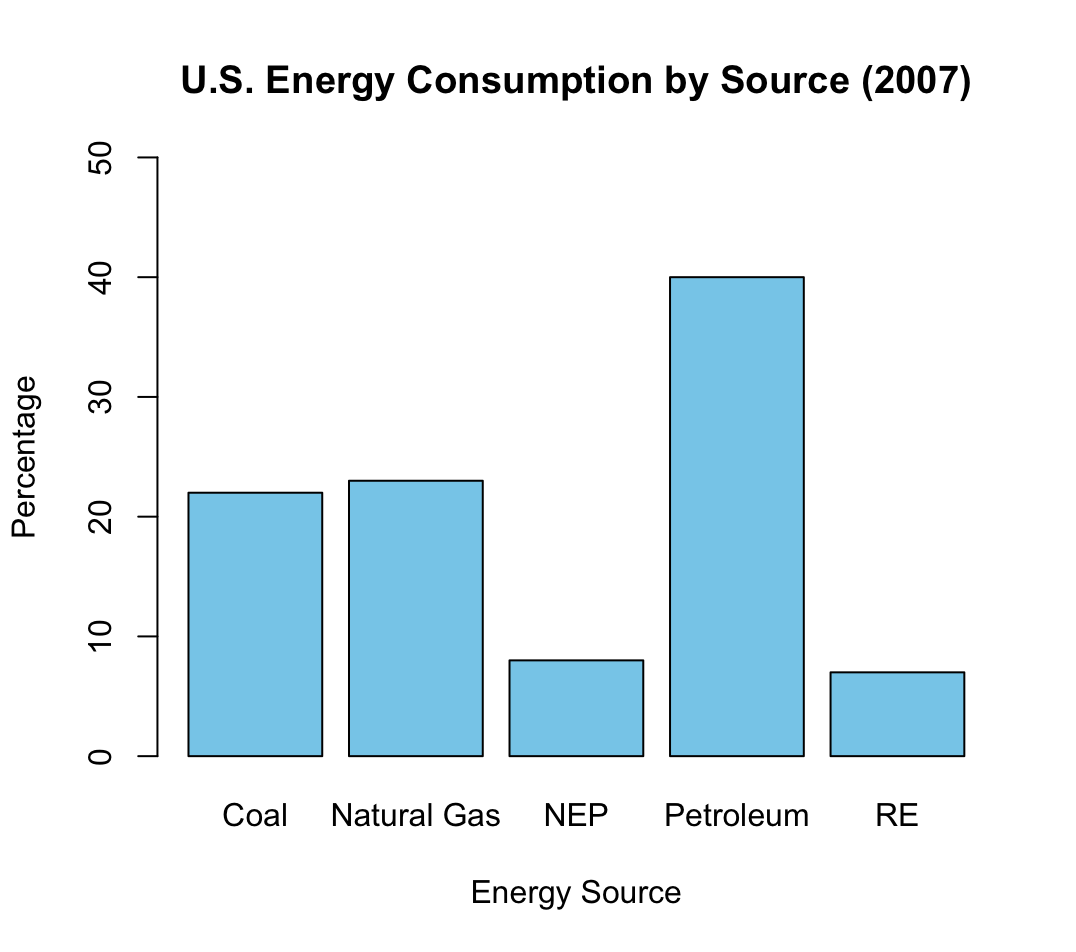
\includegraphics[width=0.85\textwidth]{1.4.3_bar_graph.png}
\caption{Bar graph of U.S. energy consumption by source (2007).}
\end{figure}

\section*{(b) Pareto Chart}
The Pareto chart ranks the energy sources from largest to smallest contribution and shows the cumulative impact.

\begin{figure}[H]
\centering
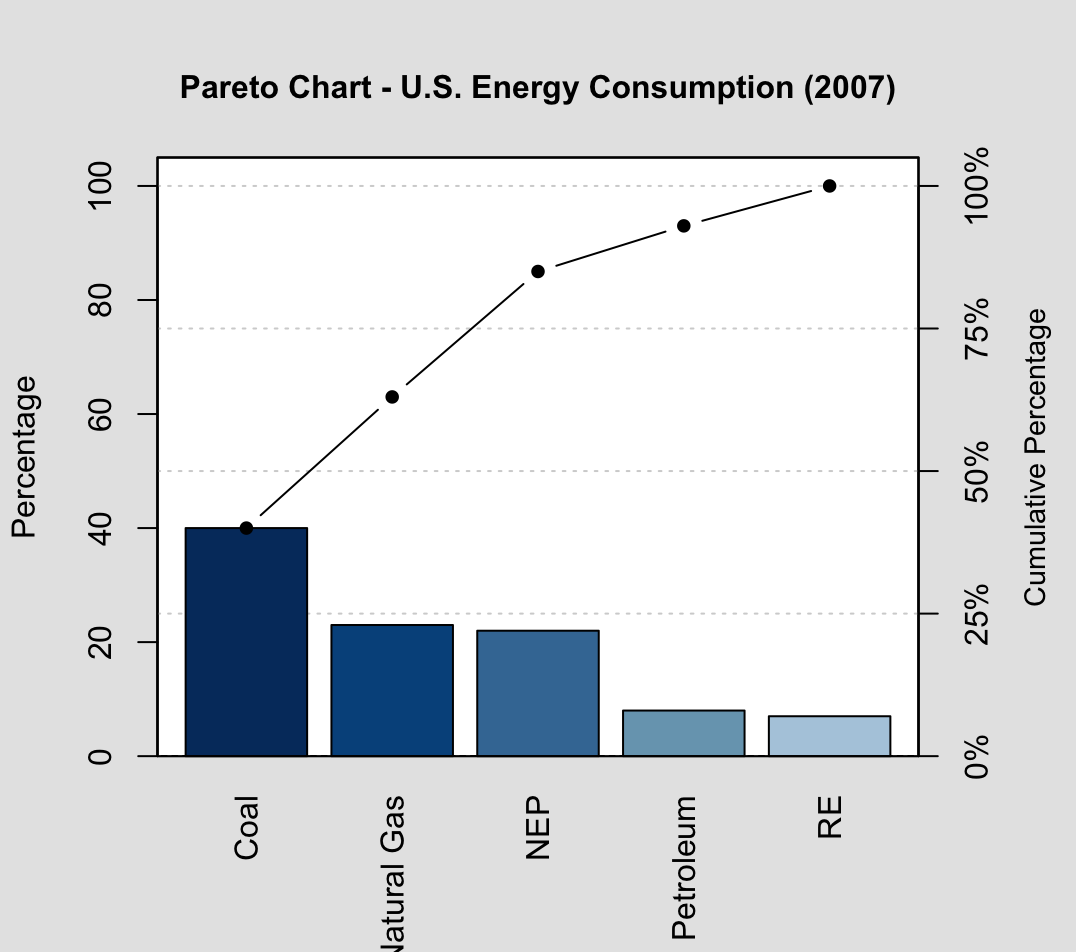
\includegraphics[width=0.85\textwidth]{1.4.3_b_pareto_chart.png}
\caption{Pareto chart of energy consumption (2007).}
\end{figure}

\section*{(c) Pie Chart}
The pie chart provides a proportional view of energy consumption distribution.

\begin{figure}[H]
\centering
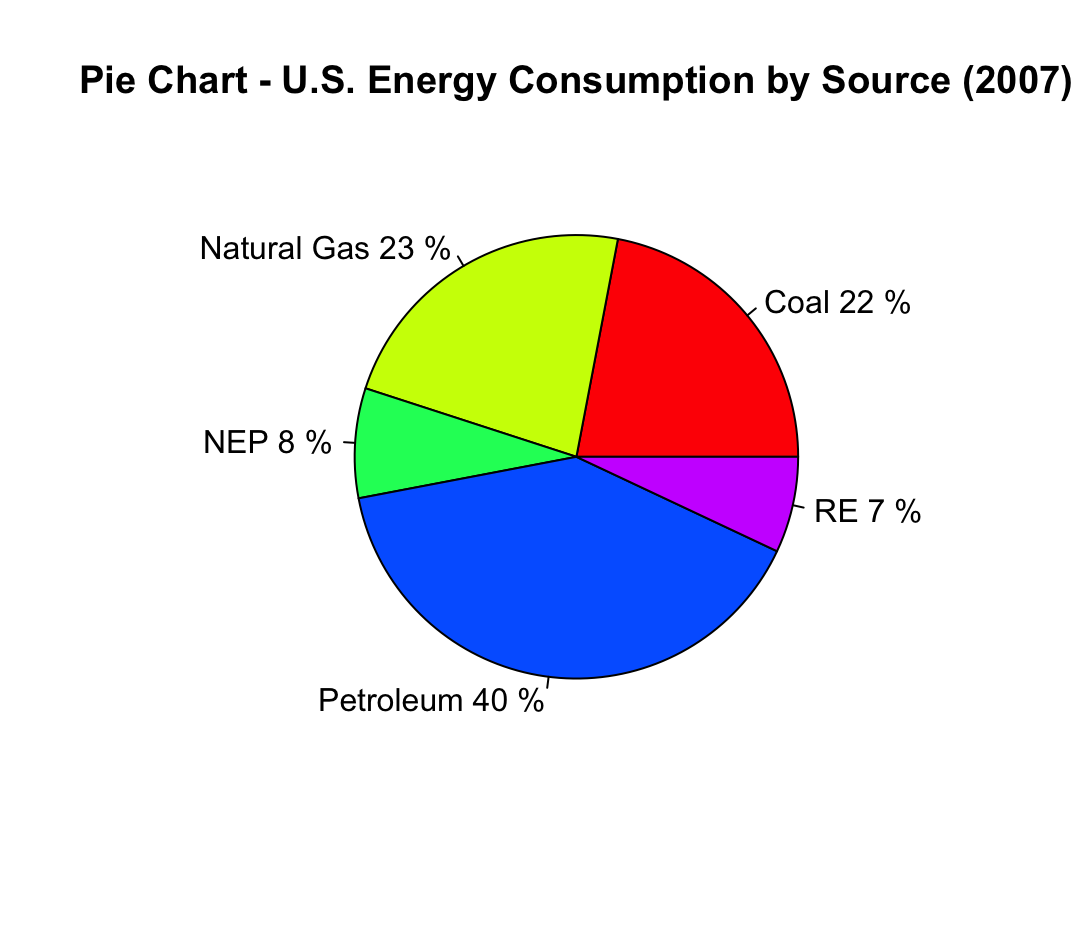
\includegraphics[width=0.85\textwidth]{1.4.3_c_pie_chart.png}
\caption{Pie chart of energy consumption (2007).}
\end{figure}

% --- Conclusion ---
\section*{Conclusion}
From the analysis, petroleum represents the largest share (40\%) of U.S. energy consumption in 2007, followed by natural gas (23\%) and coal (22\%). Renewable energy accounts for 7\%, highlighting its minor but important role in the total energy supply.

\noindent\rule{\textwidth}{0.4pt} % horizontal rule


% question 1.4.3 end

% question 1.4.14 start 

\section*{Question 1.4.14}
The following table gives radon concentrations in pCi/liter (picocurie per liter) obtained from 40 houses in a certain area.

\begin{table}[h!]
\centering
\renewcommand{\arraystretch}{1.2}
\begin{tabular}{|c|c|c|c|c|c|c|c|c|c|}
\hline
2.9 & 0.6 & 13.5 & 17.1 & 2.8 & 3.8 & 16.0 & 2.1 & 6.4 & 17.2 \\ \hline
7.9 & 0.5 & 13.7 & 11.5 & 2.9 & 3.6 & 6.1 & 8.8 & 2.2 & 9.4 \\ \hline
15.9 & 8.8 & 9.8 & 11.5 & 12.3 & 3.7 & 8.9 & 13.0 & 7.9 & 11.7 \\ \hline
6.2 & 6.9 & 12.8 & 13.7 & 2.7 & 3.5 & 8.3 & 15.9 & 5.1 & 6.0 \\ \hline
\end{tabular}
\end{table}

\begin{enumerate}
    \item[(a)] Construct a stem-and-leaf display.
    \item[(b)] Construct a frequency histogram and interpret.
    \item[(c)] Construct a pie chart and interpret.
\end{enumerate}

% Solution
\section*{Solution}
\subsection*{(a) Stem-and-leaf display}
Using the integer part as the stem and the first decimal digit as the leaf, the stem-and-leaf display is:

\begin{verbatim}
 0 | 5 6
 2 | 1 2 7 8 9 9
 3 | 5 6 7 8
 5 | 1
 6 | 0 1 2 4 9
 7 | 9 9
 8 | 3 8 8 9
 9 | 4 8
11 | 5 5 7
12 | 3 8
13 | 0 5 7 7
15 | 9 9
16 | 0
17 | 1 2
\end{verbatim}

Interpretation: the data range from 0.5 to 17.2, with many observations in the 2.x and 12–13.x ranges.

\subsection*{(b) Frequency histogram}
I used bin width 2 (pCi/l) with breaks at 0,2,4,\dots,18. The frequency counts per bin are:

\begin{tabular}{lr}
\toprule
Bin (pCi/l) & Count \\
\midrule
$[0,2)$   & 2 \\
$[2,4)$   & 10 \\
$[4,6)$   & 1 \\
$[6,8)$   & 7 \\
$[8,10)$  & 6 \\
$[10,12)$ & 3 \\
$[12,14)$ & 6 \\
$[14,16)$ & 2 \\
$[16,18)$ & 3 \\
\midrule
Total & 40 \\
\bottomrule
\end{tabular}

\noindent Interpretation: the modal bin is $[2,4)$ (10 observations); most values lie between 2 and 14 pCi/L, with a handful in the higher bins (up to 17.2), suggesting a slight right tail.

\begin{figure}[H]
\centering
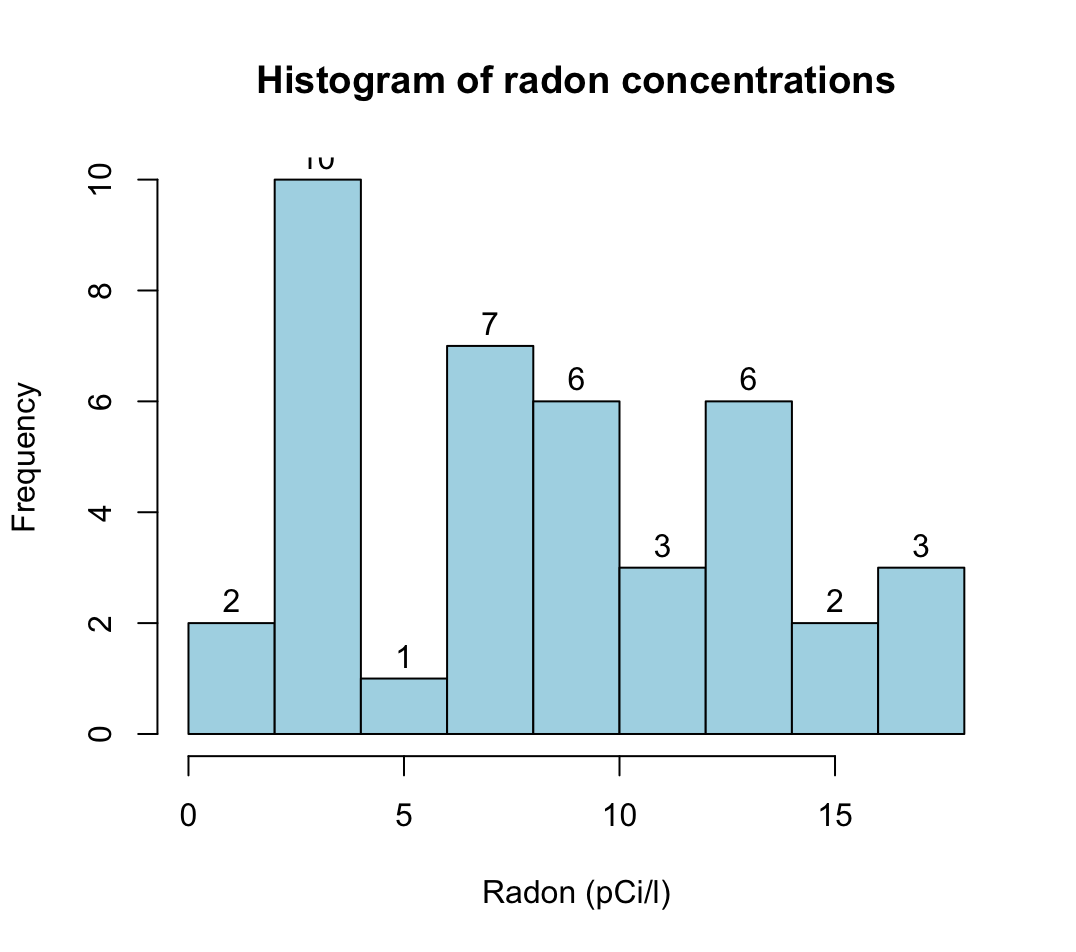
\includegraphics[width=0.85\textwidth]{1.4.14_b.png}
\caption{Histogram of radon concentrations.}
\end{figure}

\subsection*{(c) Pie chart}
I grouped the data into five ranges: $[0,4),[4,8),[8,12),[12,16),[16,18)$. Counts and percentages:

\begin{tabular}{lrr}
\toprule
Range & Count & Percent \\
\midrule
$0$--$<4$   & 12 & 30.0\% \\
$4$--$<8$   & 8  & 20.0\% \\
$8$--$<12$  & 9  & 22.5\% \\
$12$--$<16$ & 8  & 20.0\% \\
$16$--$<18$ & 3  & 7.5\% \\
\bottomrule
\end{tabular}

\medskip

Interpretation: the largest proportion (30\%) is in the lowest range (0--4 pCi/L). The middle ranges (4--16) together contain most observations; only a small fraction (7.5\%) are in 16--18 pCi/L. 

\noindent (To include the actual pie chart image, save the R plot as a PNG/PDF and include with \verb|\includegraphics{...}|)

\begin{figure}[H]
\centering
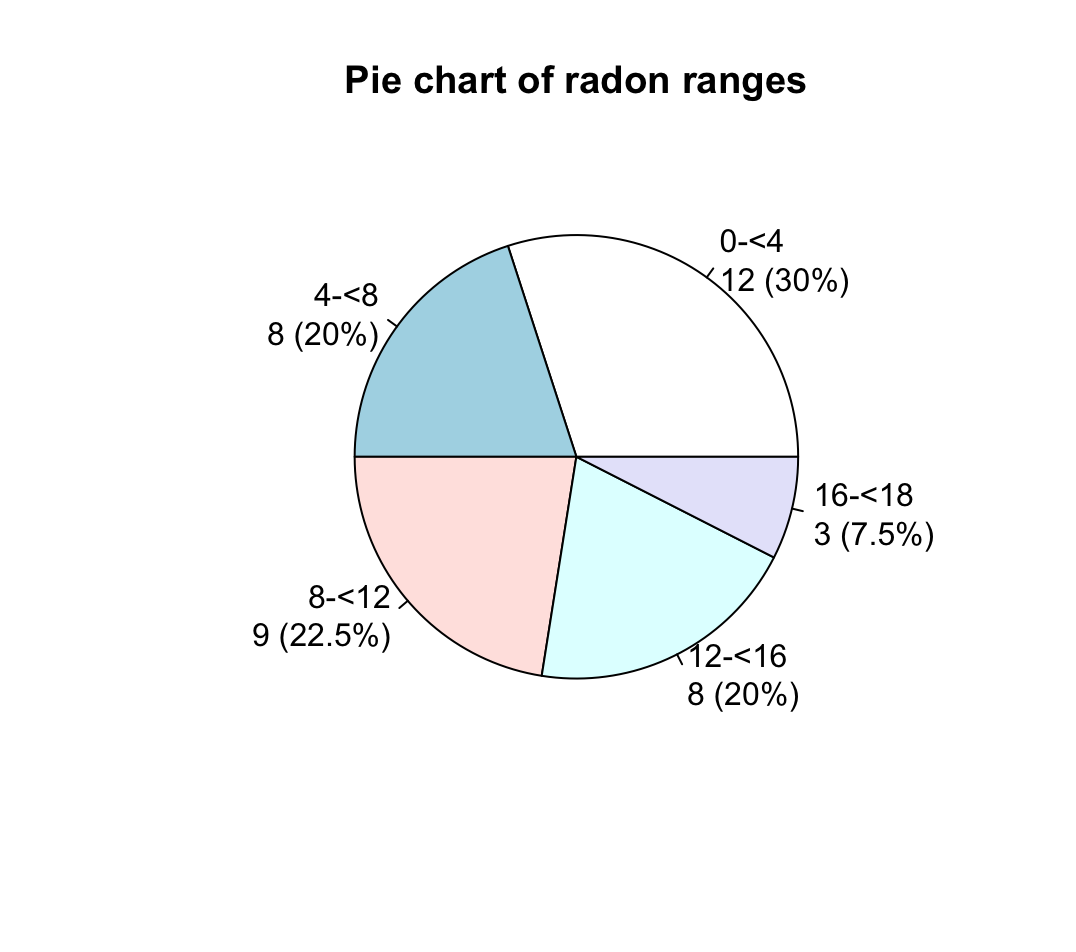
\includegraphics[width=0.85\textwidth]{1.4.14_c.png}
\caption{Pie chart of radon concentrations.}
\end{figure}

\noindent\rule{\textwidth}{0.4pt} % horizontal rule

% question 1.4.14 end

% question 1.5.5 start

\section*{Question 1.5.5}
Maximal static inspiratory pressure (PImax) is an index of respiratory muscle strength. 
The following data show the measure of PImax (cm H$_2$O) for 15 cystic fibrosis patients.

\[
\begin{array}{cccccccc}
105 & 135 & 80 & 105 & 115 & 45 & 95 & 115 \\
100 & 40 & 85 & 115 & 90 & 95 & 70 &
\end{array}
\]

\begin{enumerate}
    \item[(a)] Find the lower and upper quartiles, median, and interquartile range. 
    Check for any outliers and interpret.
    
    \item[(b)] Construct a box plot and interpret.
    
    \item[(c)] Are there any outliers?
\end{enumerate}

% Solution
\section*{Solution}

\begin{enumerate}
    \item[(a)] \textbf{Find the lower and upper quartiles, median, and interquartile range. Check for any outliers and interpret.}
    
    \vspace{0.5em}
    First, arrange the data in ascending order:
    \[
    40,\, 45,\, 70,\, 80,\, 85,\, 90,\, 95,\, 95,\, 100,\, 105,\, 105,\, 115,\, 115,\, 115,\, 135
    \]
    
    The number of observations is $n = 15$.
    
    \[
    Q_2 = \text{Median} = 8^{\text{th}} \text{ observation} = 95
    \]
    
    The lower half (below the median) is:
    \[
    40,\, 45,\, 70,\, 80,\, 85,\, 90,\, 95
    \]
    So,
    \[
    Q_1 = 4^{\text{th}} \text{ observation} = 80
    \]
    
    The upper half (above the median) is:
    \[
    100,\, 105,\, 105,\, 115,\, 115,\, 115,\, 135
    \]
    Hence,
    \[
    Q_3 = 4^{\text{th}} \text{ observation in upper half} = 115
    \]
    
    Therefore, the interquartile range is:
    \[
    IQR = Q_3 - Q_1 = 115 - 80 = 35
    \]
    
    To check for outliers, we use:
    \[
    \text{Lower Bound} = Q_1 - 1.5(IQR) = 80 - 1.5(35) = 27.5
    \]
    \[
    \text{Upper Bound} = Q_3 + 1.5(IQR) = 115 + 1.5(35) = 167.5
    \]
    
    Since all data values are between 40 and 135, there are \textbf{no outliers}.
    
    \vspace{0.5em}
    \textit{Summary:}
    \[
    Q_1 = 80, \quad Q_2 = 95, \quad Q_3 = 115, \quad IQR = 35
    \]

    \item[(b)] \textbf{Construct a box plot and interpret.}
    
    The box plot will extend from the minimum value (40) to the maximum (135), 
    with the box spanning from $Q_1 = 80$ to $Q_3 = 115$ and a median line at $95$.

    \begin{figure}[H]
    \centering
    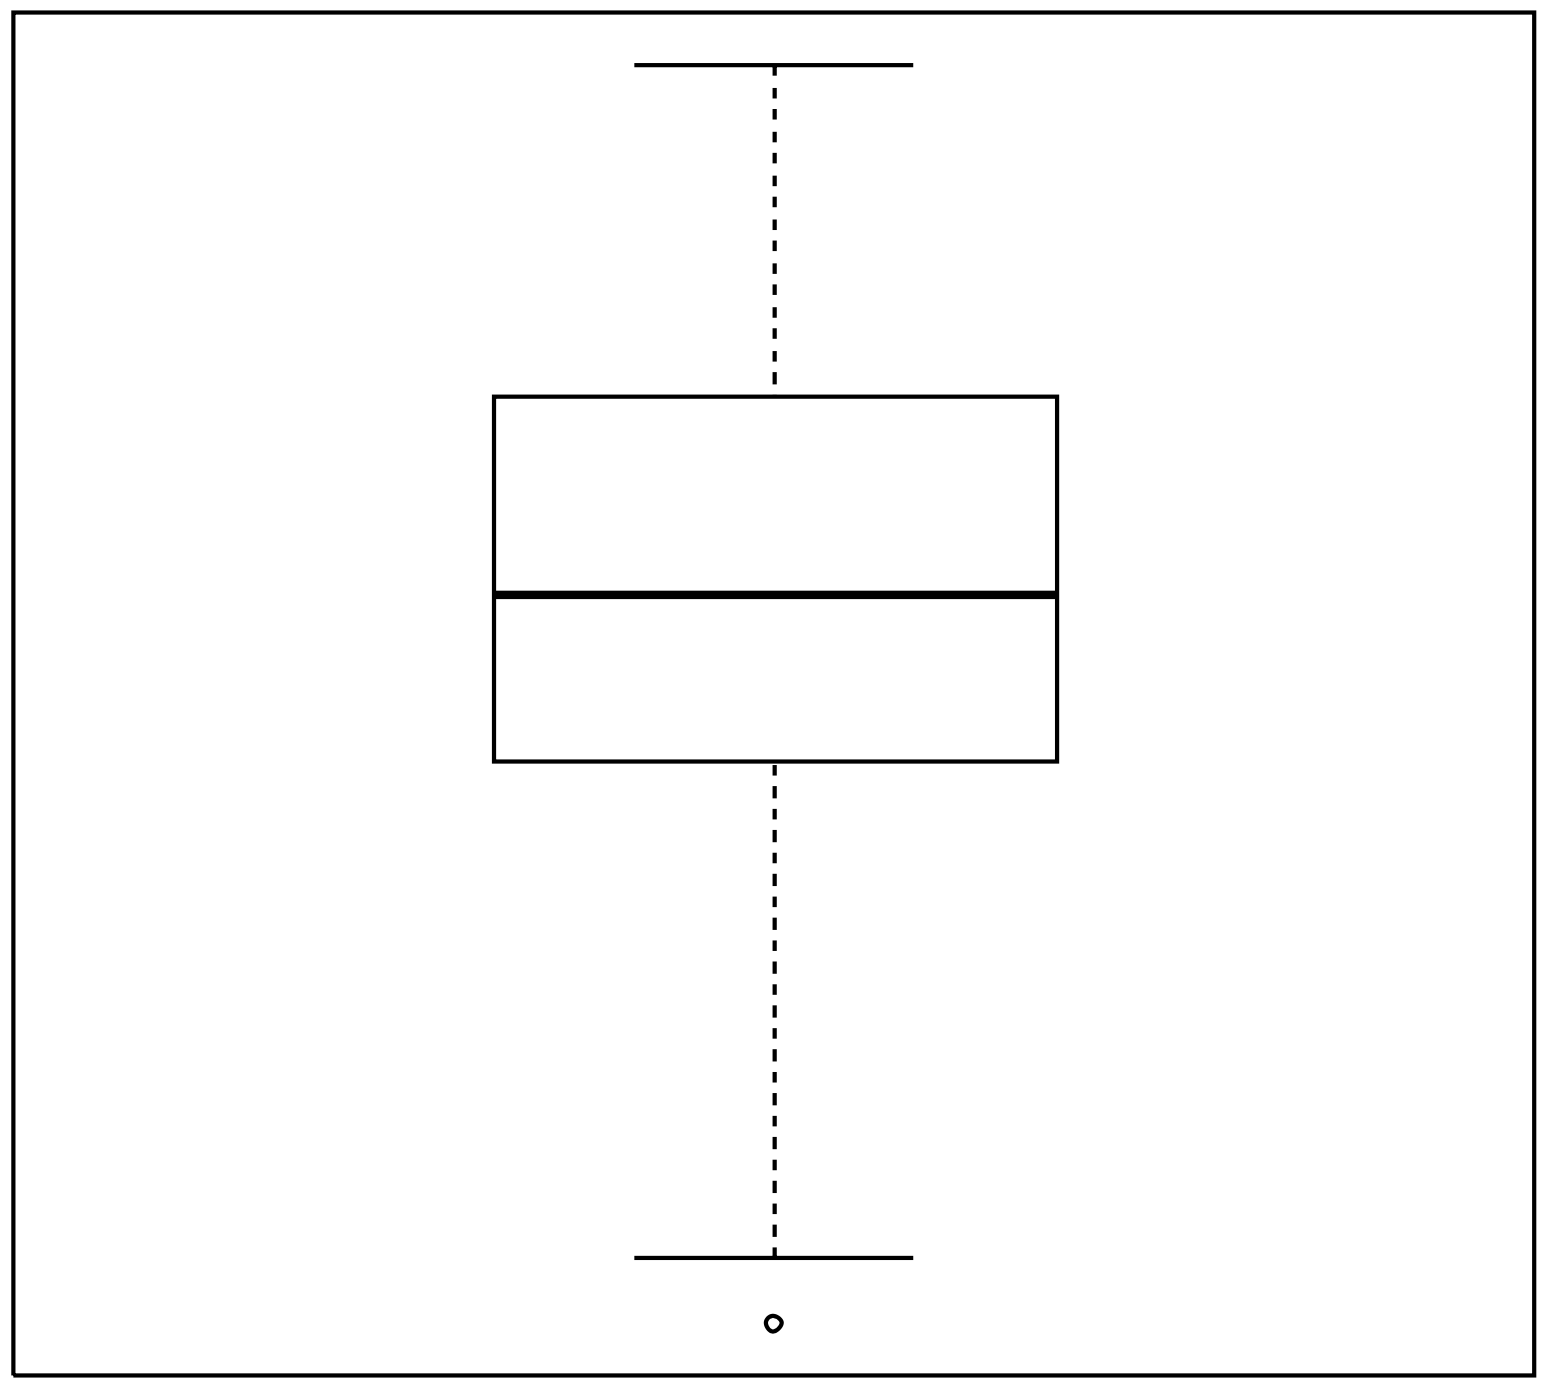
\includegraphics[width=0.6\textwidth]{box_plot.png}
    \caption{Box plot of PImax values for cystic fibrosis patients.}
    \end{figure}
    
    \vspace{0.5em}
    \textit{Interpretation:}  
    The distribution of PImax values is slightly right-skewed since the upper whisker (115–135) is longer than the lower whisker (40–80). 
    Most patients have PImax values between 80 and 115 cm H$_2$O.

    \item[(c)] \textbf{Are there any outliers?}
    
    No, there are no outliers since all observations fall within the acceptable range of 27.5 to 167.5 cm H$_2$O.
\end{enumerate}

% question 1.5.5 end
\noindent\rule{\textwidth}{0.4pt} % horizontal rule

% question 1.5.7 start
\section*{Question 1.5.7}
\begin{enumerate}
    \item[(a)] For any grouped data with $l$ classes with group frequencies $f_i$ and class midpoints $m_i$, show that
    \[
    \sum_{i=1}^{l} f_i (m_i - \bar{x}) = 0.
    \]

    \item[(b)] Verify this result for the data given in \textit{Exercise 1.5.6}.
\end{enumerate}

\textbf{Given:} Classes $0$--$4$, $5$--$9$, $10$--$14$, $15$--$19$, $20$--$24$ with frequencies
\[
f_i = 5,\;14,\;15,\;10,\;6.
\]
Class midpoints:
\[
m_i = 2,\;7,\;12,\;17,\;22.
\]

% Solution
\section*{Solution}


\subsection*{(a)}
\[
\sum_{i=1}^l f_i(m_i-\bar{x})
= \sum_{i=1}^l f_i m_i - \sum_{i=1}^l f_i\bar{x}
= \sum_{i=1}^l f_i m_i - \bar{x}\sum_{i=1}^l f_i
= n\bar{x} - n\bar{x} = 0,
\]
since $\bar{x}=\dfrac{\sum_i f_i m_i}{\sum_i f_i}$ and $\sum_i f_i=n$.

\subsection*{(b)}
Using the data from Exercise 1.5.6: $m_i = 2,7,12,17,22$, $f_i = 5,14,15,10,6$, and $\bar{x}=11.8$.
\[
\begin{aligned}
5(2-11.8) &= -49.0,\\
14(7-11.8) &= -67.2,\\
15(12-11.8) &= 3.0,\\
10(17-11.8) &= 52.0,\\
6(22-11.8) &= 61.2,
\end{aligned}
\]
and their sum equals $0$, verifying the identity numerically.

\noindent\rule{\textwidth}{0.4pt} % horizontal rule

% question 1.5.7 end

% question 1.5.10 start
\section*{Question 1.5.10}
The radon concentration (in pCi/liter) data obtained from 40 houses in a certain area are given below.\\[6pt]

\begin{table}[h!]
\centering
\renewcommand{\arraystretch}{1.2}
\begin{tabular}{|c|c|c|c|c|c|c|c|c|c|}
\hline
2.9 & 0.6 & 13.5 & 17.1 & 2.8 & 3.8 & 16.0 & 2.1 & 6.4 & 17.2 \\ \hline
7.9 & 0.5 & 13.7 & 11.5 & 2.9 & 3.6 & 6.1 & 8.8 & 2.2 & 9.4 \\ \hline
15.9 & 8.8 & 9.8 & 11.5 & 12.3 & 3.7 & 8.9 & 13.0 & 7.9 & 11.7 \\ \hline
6.2 & 6.9 & 12.8 & 13.7 & 2.7 & 3.5 & 8.3 & 15.9 & 5.1 & 6.0 \\ \hline
\end{tabular}
\end{table}

\begin{enumerate}
    \item[(a)] Find the mean, variance, and range for these data.
    \item[(b)] Find lower and upper quartiles, median, and interquartile range. Check for any outliers.
    \item[(c)] Construct a box plot.
    \item[(d)] Construct a histogram and interpret.
    \item[(e)] Locate on your histogram $\bar{x}$, $\bar{x} \pm s$, $\bar{x} \pm 2s$, and $\bar{x} \pm 3s$. Count the data points in each of the intervals 
    $\bar{x} \pm s$, $\bar{x} \pm 2s$, and $\bar{x} \pm 3s$. How do these counts compare with the empirical rule?
\end{enumerate}

% Solution
\section*{Solution}

\subsection*{(a) Mean, variance, standard deviation, range}
Number of observations: $n=40$. Sum of data $\sum x = 333.6$.
\[
\bar{x}=\frac{\sum x}{n}=\frac{333.6}{40}=8.34.
\]
Sum of squared deviations: $\sum (x_i-\bar{x})^2 = 944.376$.
Sample variance (using $n-1$):
\[
s^2=\frac{\sum (x_i-\bar{x})^2}{n-1}=\frac{944.3759999999999}{39}\approx 24.21476923.
\]
Sample standard deviation:
\[
s=\sqrt{s^2}\approx 4.92085046.
\]
Range:
\[
\max(x)-\min(x)=17.2-0.5=16.7.
\]

\subsection*{(b) Quartiles, median, IQR, outlier check}
Using interpolation (R type = 7) we obtain
\[
Q_1 = 3.675,\qquad Q_2 = 8.10,\qquad Q_3 = 12.425.
\]
\[
\mathrm{IQR} = Q_3 - Q_1 = 8.75.
\]
1.5·IQR fences:
\[
\text{Lower fence} = Q_1 - 1.5\cdot\mathrm{IQR} = -9.45,\qquad
\text{Upper fence} = Q_3 + 1.5\cdot\mathrm{IQR} = 25.55.
\]
All observations lie in $[0.5,17.2]\subset[-9.45,25.55]$, so there are no outliers by the 1.5·IQR rule.

\subsection*{(c) Boxplot}
Construct the box from $Q_1=3.675$ to $Q_3=12.425$ with median at $8.10$. 
Whiskers extend to the minimum $0.5$ and maximum $17.2$ (no outliers). 
The sample mean $\bar{x}=8.34$ may be plotted as a point for comparison. 
Interpretation: center $\approx 8.1$, IQR $=8.75$, slight right skew; no outliers.

\begin{figure}[H]
\centering
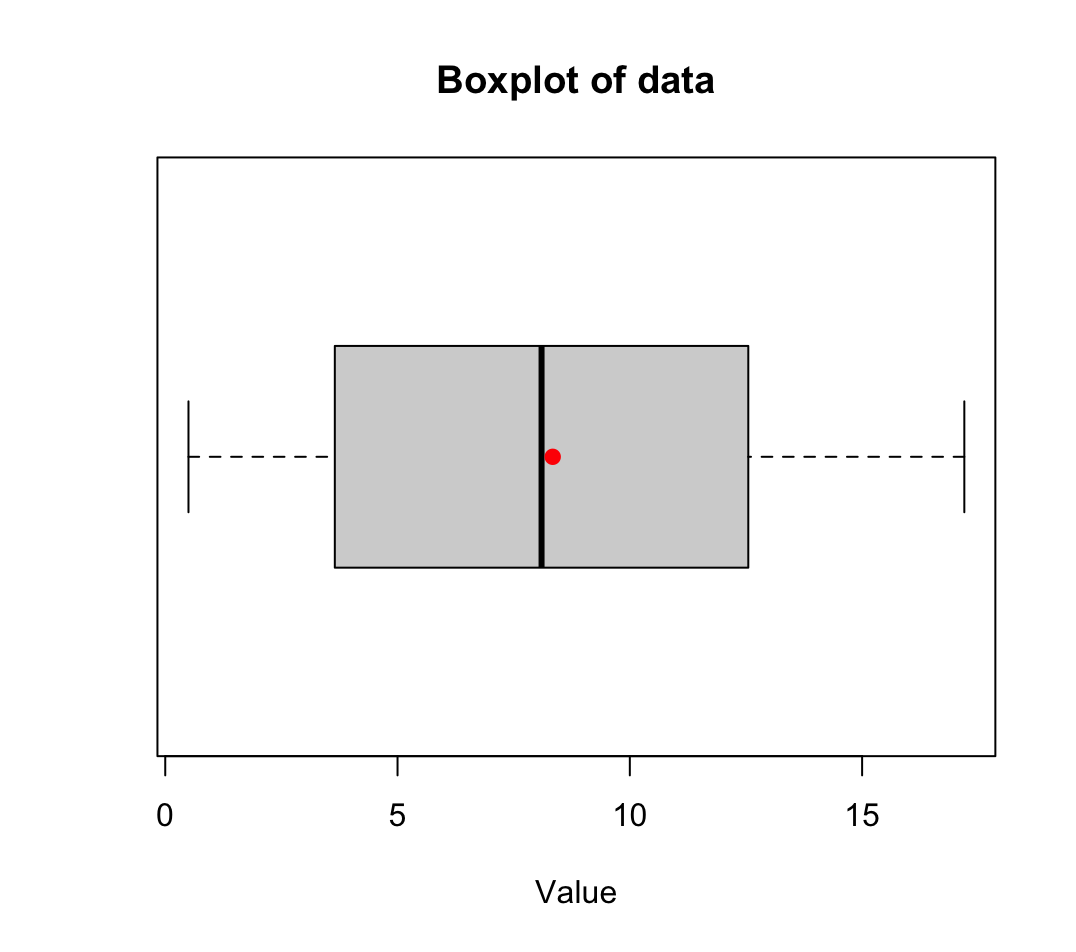
\includegraphics[width=0.6\textwidth]{1.5.10_c.png}
\caption{Box plot of radon concentration data.}
\end{figure}

\subsection*{(d) Histogram and interpretation}
Plot a histogram (e.g. using Sturges' rule) and add vertical lines for the mean $\bar{x}=8.34$ and for $\bar{x}\pm k s$ ($k=1,2,3$) to visualize spread.

Interpretation: the bulk of observations lies roughly between 3 and 13. The distribution shows a slight right skew (mean slightly larger than median). No extreme outliers are present.

\begin{figure}[H]
\centering
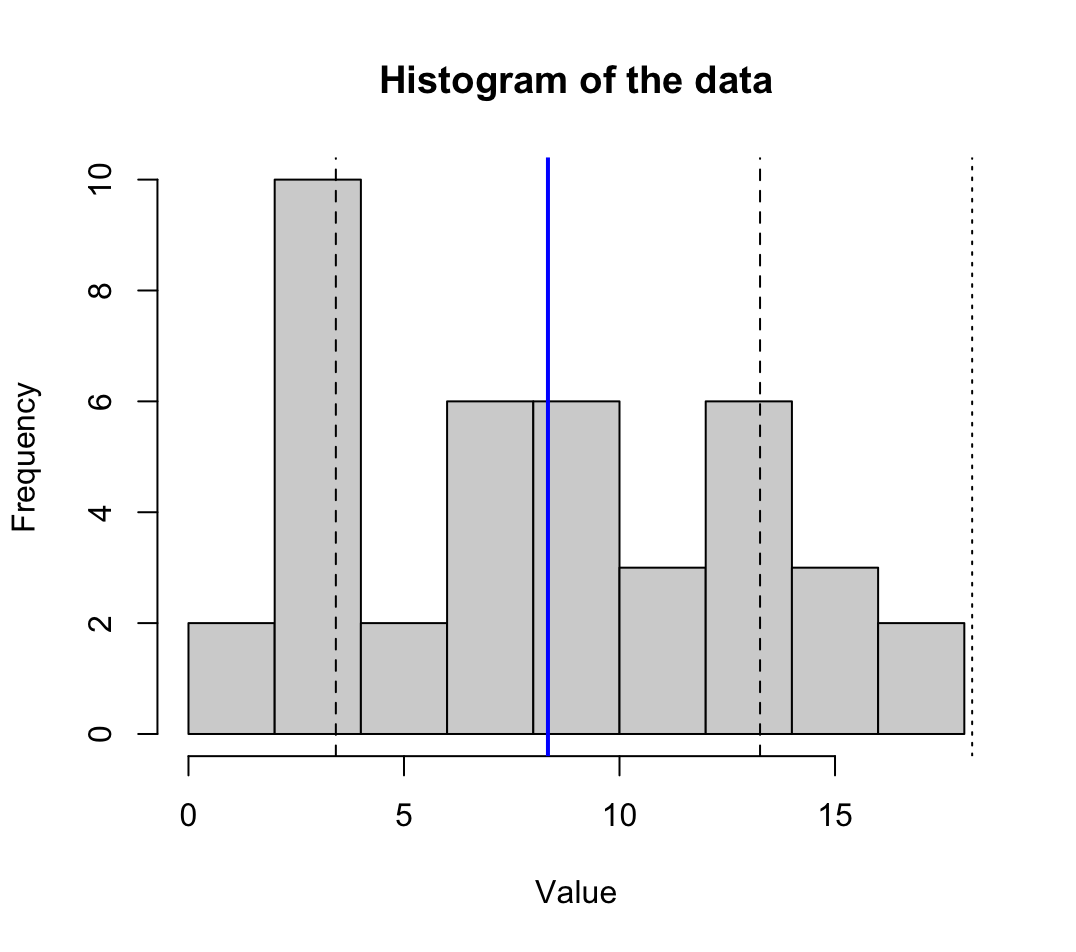
\includegraphics[width=0.85\textwidth]{1.5.10_d.png}
\caption{Histogram of radon concentration data with mean and standard deviation markers.}
\end{figure}

\subsection*{(e) Empirical-rule intervals and counts}
\[
\bar{x}=8.34,\qquad s\approx 4.92085046.
\]
\[
\bar{x}\pm s \approx [3.41915,\;13.26085],\quad
\bar{x}\pm 2s \approx [-1.5017,\;18.1817],\quad
\bar{x}\pm 3s \approx [-6.4226,\;23.1026].
\]
Counts:
\[
\text{within }\bar{x}\pm s: 24/40 = 60.0\%,\qquad
\text{within }\bar{x}\pm 2s: 40/40 = 100\%,\qquad
\text{within }\bar{x}\pm 3s: 40/40 = 100\%.
\]
Comparison with normal empirical rule (68\%, 95\%, 99.7\%): the sample has slightly fewer points within 1s and more within 2s and 3s than a normal distribution would predict.

\noindent\rule{\textwidth}{0.4pt} % horizontal rule

\end{document}
